\glsresetall
\chapter{Proposta de Virtualização e Migração de Processos para \textit{Lightweight Manycores}}
\label{chap.dev.virtualizacao}

Este trabalho de conclusão propõe-se a aumentar a independência dos processos no processador através do projeto e desenvolvimento do suporte à virtualização e migração de processos em \lws. Ambientes \cloud, nos quais o sistema de memória é de alta capacidade, usufruem da utilização de \vms para isolar duplicatas inteiras de \oss com o auxílio da virtualização a nível de instrução~\cite{sharma2016containers}. Em oposição, \lws não dispõem de centenas de GBs de memória, mas sim pequenas memórias locais. Isso associado a outras simplificações de \hardware faz com que algumas técnicas de virtualização sejam impraticáveis nesses ambientes computacionais.


Nesse contexto, visando atenuar o impacto da virtualização no sistema de memória, o presente trabalho explora um modelo de virtualização mais leve, baseado em contêineres adaptado para \lws. O \so executa os contêineres como aplicações virtuais. Sendo assim, não há a necessidade de um \os convidado, resultando em um menor impacto no sistema de memória e requisitando menor complexidade do \hardware~\cite{thalheim2018cntr, sharma2016containers}.


\section{contexto de um processo}
% \mytodo{conteinerização no nanvix}

Para o desenvolvimento da virtualização, é necessário entender o contexto de um processo no \nanvix e as relações que atrelam o processo ao \cluster e ao \so \ie as dependências que o processo tem com os recursos reais de um \cluster e com a estrutura interna do \so. De maneira geral, os módulos que compõem um processo são: \threads, \syscalls, sistema de memória e comunicação. Todos esses módulos de alguma forma têm dependências no \kernel ou \cluster. Essas dependências são ilustradas genericamente na \autoref{fig.nanvix.without-uarea} e algumas delas estão listadas abaixo:

\begin{enumerate}[label=(\roman*)]
    \item As estruturas das \threads de usuário estão armazenadas em listas internas de \kernel, assim como variáveis de sincronização (para junção de \threads, por exemplo), estruturas de escalonamento, referências às pilhas de execução e outras variáveis/estrutura de controle. É importante destacar que na abordagem inicial do \nanvix não havia separação explicita nessas estruturas para identificar quais variáveis são relacinadas a \kernel ou usuário.
    \item As estruturas responsáveis por armazenar as \syscalls, seus parâmetros e retornos requisitadas pelos \scores ao \mcore estão em espaço de \kernel.
    \item Todo o sistema de memória está armazenado no \kernel. Tabelas de diretórios, tabelas de página, \tlbs, etc.
    \item O sistema de comunicação tem dependências tanto no \kernel quanto a recursos físicos do \cluster. Os identificadores das interfaces \noc \ie de comunicação entre \clusters estão armazenadas em espaço de \kernel e referenciam uma interface física dos \clusters envolvidos na comunicação (emissor e receptor) e não aos processos envolvidos diretamente.
\end{enumerate}

Sendo assim, o desenvolvimento da virtualização nesse sistema implica no isolamento dessas dependências em um arranjo que guarde todas as informações necessárias para a execução de um processo, sejam elas manipuladas pelo usuário ou pelo \kernel. Chamamos esse arranjo de contêiner. A ideia principal é garantir que os dados incluidos no contêiner sejam suficientes para o processo executar. Isso inclui todos os dados e códigos de usuário e todas as dependências do processo com o \kernel e \cluster. Isso deve ser feito de uma maneira que permita com que o \kernel execute qualquer contêiner como uma aplicação virtual \ie deve ser possível que o contêiner se conecte ao \kernel de forma que consiga utilizar os recursos e serviços de \kernel sem que interfira em sua estrutura interna.

\begin{figure}[t]
	\centering
	
	\subcaptionminipage[fig.nanvix.without-uarea]%
                   {.4\textwidth}
                   {\os sem isolamento.}
                   {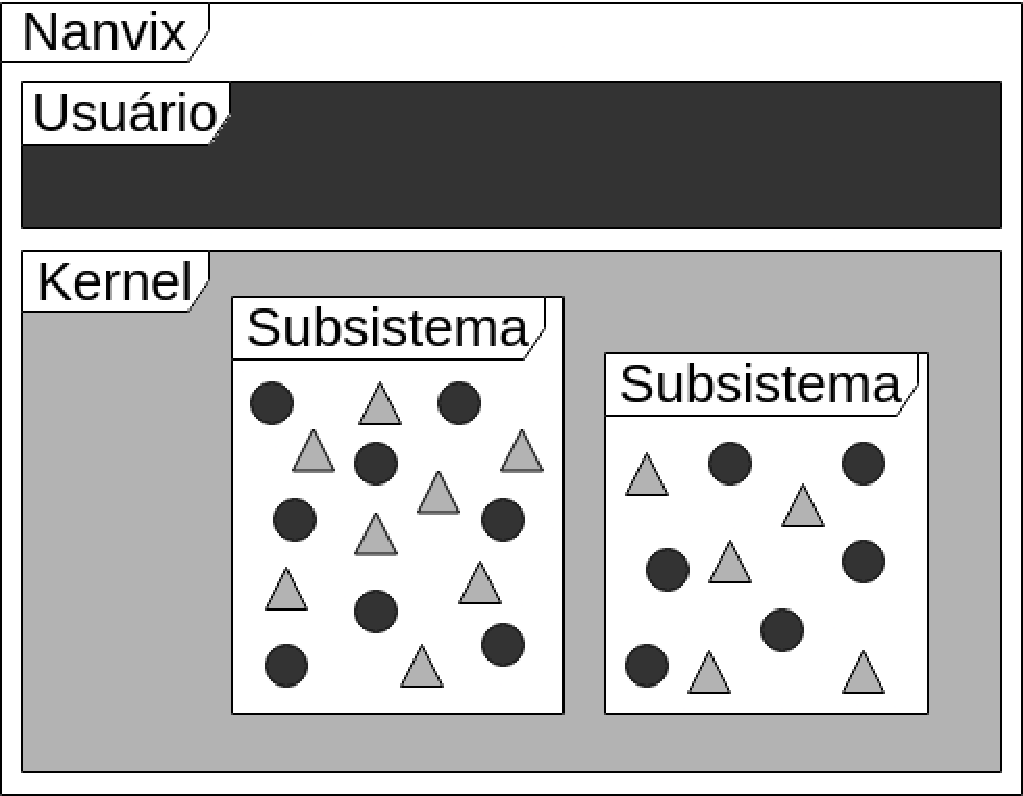
\includegraphics[width=\textwidth]{content/images/nanvix-without-uarea-uk.pdf}}
	\qquad
	\subcaptionminipage[fig.nanvix.with-uarea]
                   {.4\textwidth}
                   {\os com isolamento.}
                   {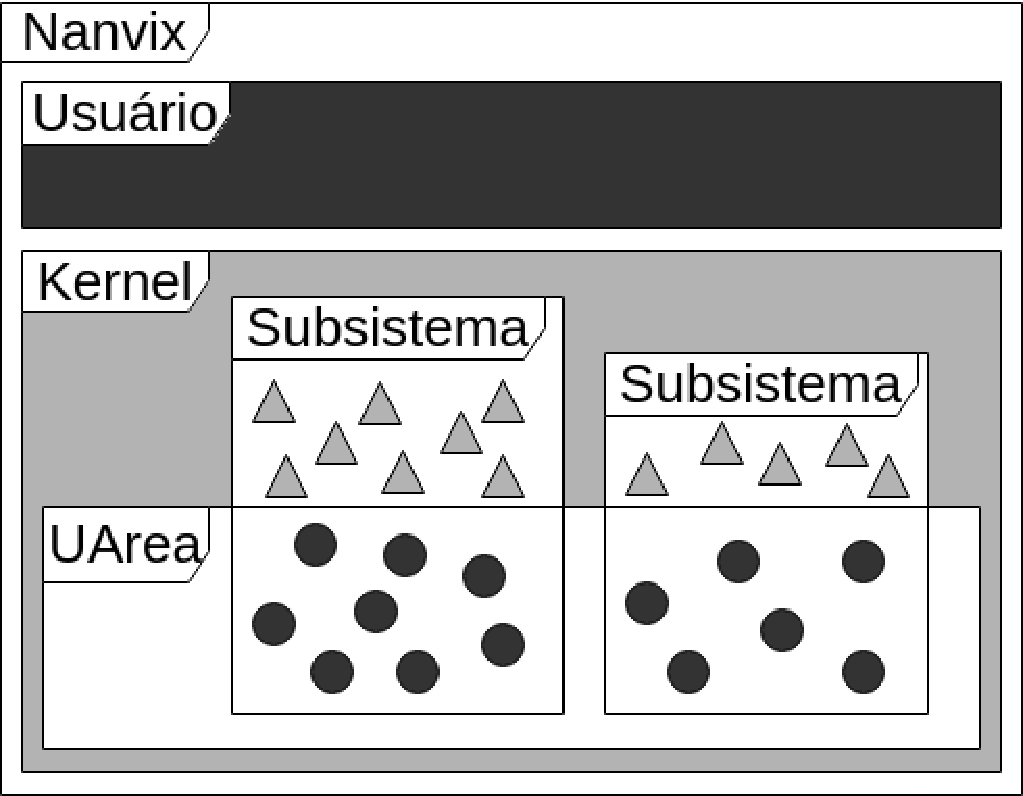
\includegraphics[width=\textwidth]{content/images/nanvix-with-uarea-uk.pdf}}

	
\includegraphics[width=.33\linewidth]{content/images/legenda.pdf}
	
	\caption{Diferença da estrutura do \nanvix com e sem a \textit{User Area}.}%
\end{figure}

\section{Isolamento do contexto de um processo de usuário}
\label{sec.dev.kernel-usuario}

Para a virtualização de processos através da conteinerização, é recomendável que as informações relevantes para a manipulação dos processos em execução estejam isoladas das informações internas do próprio \os para que os recursos de \hardware sejam utilizados de maneira eficiente~\cite{live-vm-migration-techniques}.
A \autoref{fig.nanvix.without-uarea} ilustra como os subsistemas do \nanvix são originalmente estruturados. Não há uma divisão explícita do que são dados para funcionamento interno do \os ou dependências locais do processo.
Esta abordagem torna algumas das funcionalidades do \os onerosas porque ela dificulta o acesso às informações do processo e impacta partes independentes do sistema, \eg migração e segurança dos processos.

\subsection{Divisão de Dados e Instruções}
\label{sec.divisao-dados-instrucao}

    A geração original de um executável do \nanvix compila todos os níveis em bibliotecas estáticas (\hal, \microkernel, \libnanvix, \ulibc e \multikernel) e as junta com a aplicação do usuário de forma a misturar o que é \kernel do que é usuário.
    %
    Visando a separação das informações entre usuário e \kernel, nós adaptamos o \script de ligação original do \nanvix. Na nova versão, as seções .text, .data, .bss e .rodata dos arquivos binários compilados são renomeados, especificando a qual camada de abstração tal arquivo pertence. Desta forma, é possível identificar dados e instruções de cada camada do \nanvix, assim como as informações do usuário. 
    
    Sendo assim, são geradas seções .text, .data, .rodata e .bss específicas para o \kernel e usuário. Portanto, todas as informações de \kernel, alocadas nos endereços mais baixos da memória, são isoladas das informações de aplicação, alocadas nos endereços mais altos da memória. Neste processo, são exportadas algumas constantes que apontam onde começam e terminam as partes do binário que são relacionadas ao \kernel e à aplicação \eg \textit{\_\_KERNEL\_TEXT\_START}, \textit{\_\_KERNEL\_TEXT\_END}, \textit{\_\_USER\_DATA\_START}, \textit{\_\_USER\_START}, etc. Essas constantes permitem a manipulação e gerenciamento mais precisos dos segmentos de memória do \kernel e da aplicação.
    
    Essa estratégia, além de garantir o isolamento do binário de \kernel e usuário, faz com que todos os \clusters passam a ter a mesma organização interna de \kernel, haja vista que a compilação é estática. Nesse cenário, a migração pode ser feita parcialmente através do salvamento dos dados e instruções da aplicação de um \cluster, os quais estão contidos no intervalo identificado pelas constantes, e restauração destes nas respectivas posições \ie no mesmo intervalo em outro \cluster. Com isso, evita-se manipulações mais complexas do processo como a busca em várias regiões de memória para montar o estado interno do processo.

    % \mytodo{colocar alguma parte do linker?}
    % \mytodo{Souto: ngm vai entender o código do linker mas seria legal colocar e discutir melhor sobre as constantes.}
    
\subsection{\textit{User Area}}
\label{sec.uarea}

    Além da separação de dados e instruções entre \kernel e aplicação, é necessário a identificação e separação das estruturas internas do \so que são manipuladas pelo usuário e constituem o estado interno do processo. Nesse contexto, é introduzido o conceito de conteinerização para isolar as dependências que o usuário possui dentro do \cluster. Ou seja, nós isolamos os dados que são gerenciados pelo \kernel mas pertencem ao contexto do processo de usuário. Neste contexto, nós isolamos tais dados em uma região de memória bem definida, denominada de \uarea. 

    Detalhadamente, a \uarea mantém informações sobre:
    \begin{enumerate}[label=(\roman*)]
        \item \Threads ativas, incluindo identificadores, pilhas de execução e contextos;
        \item Filas de escalonamento de \threads;
        \item Variáveis de controle interno do sistema de \threads, como quantidade de \threads ativas;
        \item Tabela de gerenciamento de chamadas de sistema; e
        \item Estruturas de gerenciamento de memória \eg sistema de paginação
    \end{enumerate}

    Essa estrutura genérica foi projetada para englobar as várias arquiteturas suportadas pelo \nanvix. Além disso, a estrutura permite a modificação e expansão, não se limitando ao estado atual do desenvolvimento do \nanvix, para atender os objetivos de outros projetos que usufruam do \nanvix.

\section{Conteinerização}
O uso de contêineres faz-se presente neste trabalho, porém seu funcionamento difere das abordagens convencionais. De maneira geral, nas perspectivas tradicionais, um contêiner é uma estrutura responsável por isolar do \so a execução de uma aplicação que roda sob seus limites. Esta estrutura geralmente é construída a partir de uma imagem base de um \so, na qual podem ser instaladas novas bibliotecas ou ferramentas, de modo a permitir a customização do ambiente de execução da aplicação de acordo com as necessidades do usuário. Sendo assim, o contêiner pode executar um \so diferente de onde está sendo executado e também pode conter ferramentas/bibliotecas diferentes ou em uma versão diferente das do \so que executa o contêiner.

Em contraste, a proposta neste trabalho utiliza o conceito de contêiner de uma maneira diferente. A proposta neste trabalho é apenas isolar o processo do \kernel e do \cluster que o executa a fim de permitir maior mobilidade do processo no processador. Sendo assim, os contêineres não contêm imagens de \so distintas ou funcionalidades diferentes uns dos outros. Todos os contêineres executam sobre a mesma estrutura de \kernel (que é idêntica em todos os \clusters do \lw), apenas se diferenciando pelo estado interno do processo que está sendo executado \eg quantidade de \threads criadas, dados manipulados pelo usuário, espaços de memória alocados dinamicamente, etc.

Nesse cenário, um contêiner neste trabalho pode ser definido como a junção do código de usuário, dados de usuário e \uarea. Essa união abrange todo o essencial para a execução do processo: código e dados de usuário; e as dependências internas do processo no \cluster que o executa.


\section{Migração de Processos}
\label{sec.migracao}

Como aplicação direta do isolamento do processo, conseguida através da virtualização com os contêineres, a migração de processos torna-se mais palpável. Especificamente, nós eliminamos a necessidade de descobrir quais são e onde estão as informações que compõem o estado de um processo dentro do \nanvix porque tudo está isolado via conteinerização, facilitando a transferência de seu contexto. Isso só é possível porque os \clusters possuem uma estrutura de \kernel idêntica (devido às mudanças desenvolvidas no processo de compilação detalhados na \autoref{sec.divisao-dados-instrucao}). Por este motivo, eliminamos o envio de dados redundantes entre \clusters referentes à instância local do \os, atenuando o impacto da migração sobre a \noc.

\subsection{Rotina de migração}
\label{sec.rotina-migracao}

Para a migração de um processo entre \clusters foi desenvolvida uma rotina de migração. A funcionalidade é similar ao \criu, ferramenta utilizada por \softwares de gerenciamento de contêineres como o Docker. Porém, a migração é executada por intermédio de \daemons do \os. Neste projeto, foi implementado o algoritmo \hotmigration, em que a aplicação é migrada enquanto é executada, como detalhado na \autoref{sec.hotmigration} utilizando a técnica \precopy visto na \autoref{sec.precopymigration}. De forma resumida, a aplicação é migrada durante sua execução, sendo restaurada no \cluster destinatário após a transferência completa dos dados do contêiner. A seguir é detalhado como funciona o \daemon e o fluxo de migração.

\subsubsection{\Daemon de Migração}

O \daemon de migração é inicializado durante o \boot do sistema. Resumidamente, o \daemon é composto por um fluxo de \tasks, as quais são inicializadas e conectadas durante a inicialização do módulo de migração, que ocorre durante o \boot. Além disso, nesse período ainda é criada a porta de \mailbox por onde o \daemon recebe as requisições de migração.
    
O fluxo de migração de inicia com o recebimento de uma requisição de migração. Quando uma requisição é detectada \ie quando é lida uma mensagem de migração da porta específica do \daemon, a \task principal do \daemon (o \handler do \daemon de migração) é ativa. Esta função é responsável por interpretar a mensagem recebida. É neste momento em que os \clusters envolvidos são identificados \ie é reconhecido qual é o \cluster remetente e qual o \cluster destinatário. É importante destacar que tanto o \cluster remetente quanto o destinatário recebem a mesma mensagem, porém com códigos de operação diferentes. Enquanto um recebe uma mensagem com o código de envio dos dados (identificando o remetente), o outro recebe uma mensagem com o código de recebimento de dados (identificando o destinatário).

Depois da identificação dos \clusters envolvidos e seus papéis durante o procedimento, são executadas as \tasks responsáveis pela migração de fato \ie pelo envio e recebimento de dados.


\subsubsection{Fluxo de Migração}

\begin{figure}[bt]
    \centering
    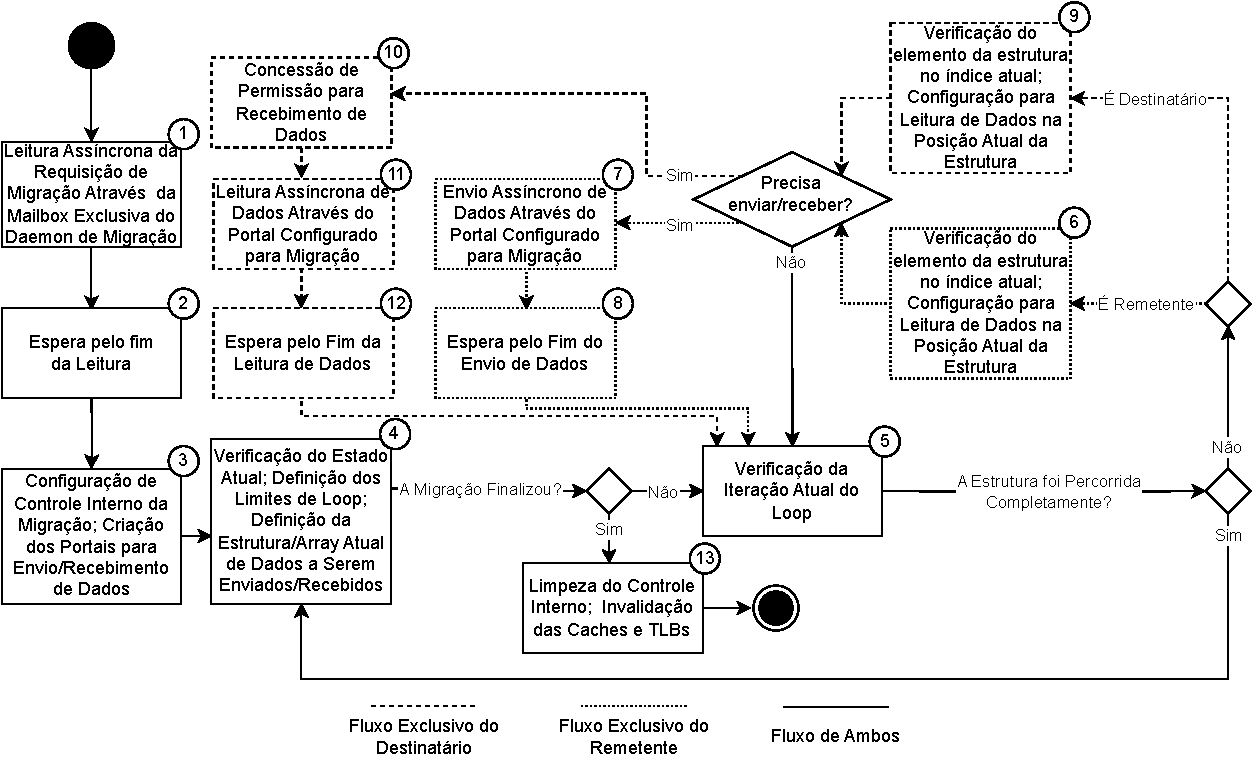
\includegraphics[width=\linewidth]{content/images/migration-steps-tasks.pdf}
    \caption{Fluxo de tasks de migração}
    \label{fig.migrationsteps}
\end{figure}

A \autoref{fig.migrationsteps} ilustra o fluxo de execução da migração. Nela, cada quadro corresponde a uma \task e a escrita que cada quadro contém indica o que a \task faz. Destaca-se que neste fluxo todas as comunicações são assíncronas. O que significa que em nenhum momento uma \task espera ativamente por uma comunicação. Isso é feito com o intuito de evitar que o sistema seja bloqueado por alguma \task que esteja esperando por uma comunicação. Dito isso, esse \design de migração baseado em \tasks foi adotado por garantir o isolamento das etapas de migração em passos bem definidos e porque o funcionamento da comunicação assíncrona está intrinsecamente ligado ao sistema de \tasks do \nanvix. Mais detalhadamente, uma comunicação assíncrona funciona da seguinte maneira: uma \task envia mensagens de tamanho fixo repetidas vezes até que se atinja a quantidade de \bytes passada como parâmetro. Quando a mensagem é enviada completamente, é enviado um sinal a outra \task, cuja função é apenas sinalizar o final de uma comunicação. As estruturas de ambas as \tasks são criadas e configuradas de acordo com a funcionalidade desejada.

Portanto, tendo em vista que a comunicação assíncrona fundamenta-se na utilização de \tasks, é natural e mais simples que o \daemon de migração seja composto por \tasks. Desse modo as \tasks de início e fim das comunicações são conectadas às \tasks de controle da migração.

Abaixo estão descritos o funcionamento mais detalhado de cada \task de migração de acordo com o número identificador ilustrado na \autoref{fig.migrationsteps}.


\begin{description}[leftmargin=*,labelwidth=!,labelindent=0pt]
    \item[1.] Esta é a \task responsável pela leitura assíncrona de uma mensagem enviada ao \daemon de migração. Esta \task é ativa no momento de \boot durante a etapa de configuração do sistema de migração e é reativada no momento em que uma migração finaliza com ou sem êxito \ie assim que uma migração finaliza seja por ter completado todo seu processo ou por ocorrência de algum erro. Isso permite que o fluxo seja reusado, o que significa que o \cluster pode atender múltiplas requisições de migração sequêncialmente independentemente do papel do \cluster (remetente ou destinatário).
    \item[2.] Esta \task é ativa no momento em que uma mensagem é lida pela \task 1. Portanto, esta é a \task responsável por sinalizar que uma mensagem foi recebida e lida.
    \item[3.] Esta é a \task que interpreta a mensagem recebida. A mensagem é composta por um código de operação que identifica o papel do cluster na migração e por dois inteiros que identificam os \clusters envolvidos na migração. Caso o \cluster seja o destinatário, durante a execução desta \task é invocada a chamada de sistema \freeze para congelar a execução do processo de usuário (neste momento o \cluster remetente já deve ter congelado sua execução também). Essa \task passa um parâmetro indicando o papel do \cluster na migração. Nas etapas posteriores esse parâmetro é decisivo na escolha dos subfluxos que o procedimento deve seguir \eg envio ou recebimento de dados.
    \item[4.] Esta \task é responsável pelo gerenciamento do estado atual do envio/recebimento de dados da migração. No total são 10 estados. Abaixo estão os estados e as estruturas que são manejadas em cada um deles:

    \begin{description}[leftmargin=!,labelwidth=\widthof{MSTATE\_FRAMES\_BITMAP \qquad}]
        \item [MSTATE\_SECTIONS] Seções do binário identificadas como partes do usuário. Particularmente, são enviadas as seções \texttt{.user.text}, \texttt{.user.data}, \texttt{.user.bss} e \texttt{.user.rodata}.
        \item [MSTATE\_UAREA] \uarea.
        \item [MSTATE\_SYSBOARD] Tabela de chamadas de sistema.
        \item [MSTATE\_PAGEDIR] Tabela de diretórios.
        \item [MSTATE\_PAGETAB] Tabela de páginas.
        \item [MSTATE\_KSTACKSIDS] Lista responsável pela identificação de quais páginas de \kernel estão sendo usadas.
        \item [MSTATE\_KSTACKSPHYS] Páginas de \kernel que estão sendo usadas.
        \item [MSTATE\_FRAMES\_BITMAP] \Bitmap responsável pela identificação de quais \frames estão sendo usados.
        \item [MSTATE\_FRAMES\_PHYS] \Frames de usuário que estão sendo usados
        \item [MSTATE\_FINISH] Não manipula estruturas. Apenas reseta o controle interno da migração e invalida as \tlbs e \caches.
    \end{description}

\end{description}
% \subsubsection{Congelamento da execução do processo em um estado consistente}
% % \begin{description}
% 	% \item[1. Congelamento da execução do processo em um estado consistente.] \hfill
	
% 	Antes do envio da aplicação a outro \cluster, é necessário que o processo esteja em um estado consistente e estático. Isso significa que durante o processo de migração é preciso que todas as operações dele sejam pausadas. Isso é feito objetivando evitar inconsistências que podem ser causadas por condições de corrida \eg impedir perda de instruções, impedir perda de retornos de chamadas de sistemas, impedir perda de sinais de sincronização, impedir inconsistência de valores de variáveis de usuário, etc. 
    
%     Para atingir esse estado consistente, foi criada a chamada de sistema \freeze, a qual é invocada no início do processo de migração. Esta é uma chamada de sistema que é tratada apenas pelo \mcore. Especificamente, esta chamada ativa uma variável interna do \so que impede o escalonamento de \threads de aplicação (\threads que não executam no \mcore) e envia um sinal de reescalonamento para todos os \scores, para que as \threads de usuário saiam de execução o mais rápido possível. Isso garante uma pausa na aplicação sem que o \so seja impedido de executar, o que é imprescindível para a migração, já que as informações do processo precisam ser enviadas pelas interfaces \noc do \cluster remetente, o que exige que o \so atenda às requisições de envio de dados. Isso só é possível se as \threads de sistema continuarem a ser executadas apesar do congelamento das de usuário.
    
%     Após o travamento no escalonamento de \threads de usuário, novas chamadas de sistema requisitadas pela aplicação não podem ocorrer. Sendo assim, após a migração, o \cluster destinatário atenderá às chamadas não atendidas e reconhecerá as atendidas, pois as estruturas de sincronização e variáveis de retorno são migradas também durante o processo. Após o congelamento do escalonamento e a retirada das \threads de usuário dos \scores, o processo é considerado consistente e seu contexto está apto para ser migrado.

% \subsubsection{Transferência do Contexto do Processo entre \Clusters}
% 	% \item[2. Transferência do contexto do processo entre \clusters.] \hfill
	
% 	Com o processo em um estado consistente, uma série de \tasks de sistema, que são escalonadas no \mcore, são executadas para o envio dos dados ao \cluster destinatário. O envio é feito através das abstrações de comunicação \mailbox e \portal. O envio de dados, instruções e \uarea garantem que o contexto inteiro do processo seja enviado, possibilitando a retomada da execução no \cluster destinatário.

	
% \subsubsection{Restauração da Execução do Processo no \Cluster de Destino}
%     % \item[3. Restauração da execução do processo no \cluster destino.] \hfill
	
% 	Com o contexto do processo já no \cluster destinatário, a execução é restaurada. Isso é feito pela chamada de sistema \unfreeze, que descongela o escalonamento de \threads de usuário. Assim, a execução do processo continua normalmente, agora em outro \cluster.
% \end{description}

\mytodo{detalhar como funcionam as tasks e threads em cada cluster: remetente e destinatario}
\mytodo{como funciona a migração para um cluster com nenhum processo alocado}